\chapter{Результаты исследований}\label{ch:ch7}

\section{Минеральный состав}

Минеральный состав исследуемых грунтов был определен путем проведения рентгено-структурного 
анализа, который был сделан работниками кафедры  инженерной и экологической геологии 
геологического факультета МГУ им.М.В.Ломоносова
инж. 1 кат. С.А. Гараниной, вед. инж. С.В. Закусиным, ст.н.с., к.г.-м.н. В.В. Крупской.
Рентгеновские дифракционные картины представлены в приложении 1.

По результатам анализа была составлена таблица \ref{tab:mineral}, отражающая минеральный состав 
исследованных грунтов.


\begin{table}[]
  \small
    \centering
  \begin{threeparttable}
  \caption{Минеральный состав (вес. \%)}
  \label{tab:mineral}
    \begin{tabular}{|l|c|c|c|c|c|c|}
        \hline
                                  & GJ68B7 & GJ68D4 & GJ6881 & GJ6890 & GJ6898 & GJ6899 \\ \hline
    Хлорит                        & 1,9  & 3,9  & 2,3  & 2,9  & 2,4  & 1,4  \\ \hline
    Смектит*                      & 14,3 & 13,2 & 34,7 & 32,9 & 22,0 & 15,0 \\ \hline
    Иллит                         & 8,8  & 4,8  & 5,9  & 4,3  & 5,2  & 6,2  \\ \hline
    Палыгорскит**                 & 1,0  & 0,1  & 0,0  & 0,0  & 0,0  & 0,0  \\ \hline
    Каолинит                      & 3,6  & 1,9  & 2,8  & 1,8  & 1,1  & 2,7  \\ \hline
    Кварц                         & 44,1 & 53,0 & 35,0 & 40,1 & 47,4 & 48,7 \\ \hline
    КПШ (микроклин, ортоклаз)     & 8,7  & 9,0  & 8,7  & 5,6  & 11,9 & 14,4 \\ \hline
    Плагиоклазы (альбит, андезит) & 3,3  & 7,3  & 6,7  & 11,5 & 7,9  & 8,4  \\ \hline
    Кальцит                       & 6,2  & 2,1  & 0,8  & 0,3  & 0,0  & 0,4  \\ \hline
    Доломит                       & 7,7  & 2,9  & 1,1  & 0,2  & 0,0  & 0,0  \\ \hline
    Сидерит                       & 0,0  & 0,0  & 0,0  & 0,0  & 0,3  & 0,4  \\ \hline
    Рутил                         & 0,0  & 0,0  & 0,4  & 0,4  & 0,0  & 0,9  \\ \hline
    Пирит                         & 0,4  & 0,3  & 0,3  & 0,0  & 0,4  & 0,4  \\ \hline
    Амфиболиты (роговая обманка)  & 0,0  & 1,5  & 1,3  & 0,0  & 1,4  & 1,1  \\ \hline
    \end{tabular}
    \raggedright 
    * Вероятно присутствие смешанослойного минерала иллит-смектит с~преобладанием смектитовых 
    (набухающих) пакетов. 
    Для точной диагностики требуется выделение глинистой фракции.
    \\
    ** Присутствие палыгорскита требует уточнения путем анализа глинистой фракции
    \end{threeparttable}
    \end{table}

По данным из таблицы \ref{tab:mineral} видно, что в грунтах преобладают такие 
минералы, как кварц (среднее 44,7\%) и смектит (22\%). Напротив, минералов 
палыгорскит, сидерит, рутил и пирит практически нет ни в одном образце. 

Также в лаборатории были построены ренгеновские дифракционные 
картины, представленные в Приложении \ref{app:difrac}. 

\section{Гранулометрический состав}

Гранулометрический состав грунтов был определен ареометрическим 
методом только для песчанистой и глинистой фракций, не учитывая 
крупнообломочную фракцию. 

По результатам анализа на гранулометрический состав были 
построены интегральные (кумулятивные) кривые (рис. \ref{fig:curves}).

{
\small
\pgfplotsset{
%samples=15,
width=0.45\linewidth,
xlabel={Диаметр частиц $d$, мм},
ylabel={Содержание частиц, \%},
%extra y ticks={45},
legend pos=north west,
ymin = 0,
ymax = 100,
}

\begin{figure}
	{\centering
	\small
	\subbottom[ИГЭ-6 (суглинки тугопластичные)]{\begin{tikzpicture}
    \begin{semilogxaxis}[]
    
    % ИГЭ-6
    \addplot[smooth, no marks, red!70!orange!80!black] table [x=Size, y=GJ6805, col sep=semicolon] {data/hydrometer-cumulative.csv};
    \addplot[smooth, no marks, red!70!orange!80!black] table [x=Size, y=GJ6807, col sep=semicolon] {data/hydrometer-cumulative.csv};
    \addplot[smooth, no marks, red!70!orange!80!black] table [x=Size, y=GJ6838, col sep=semicolon] {data/hydrometer-cumulative.csv};
    \addplot[smooth, no marks, red!70!orange!80!black] table [x=Size, y=GJ6835, col sep=semicolon] {data/hydrometer-cumulative.csv};
    
    \end{semilogxaxis}
\end{tikzpicture}}
	\hfill
	\subbottom[ИГЭ-7 (суглинки тугопластичные)]{\begin{tikzpicture}
    \begin{semilogxaxis}[]
    
    % ИГЭ-7
    \addplot[smooth, no marks, lime!40!black] table [x=Size, y=GJ6898, col sep=semicolon] {data/hydrometer-cumulative.csv};
    \addplot[smooth, no marks, lime!40!black] table [x=Size, y=GJ6874, col sep=semicolon] {data/hydrometer-cumulative.csv};
    
    \end{semilogxaxis}
\end{tikzpicture}
}
	}
	\\
	{\centering
	\small
	\subbottom[ИГЭ-8а (глины полутвердые)]{\begin{tikzpicture}
    \begin{semilogxaxis}[]
    
    % ИГЭ-8
    \addplot[smooth, no marks, green!10!lime!30!black] table [x=Size, y=GJ6822, col sep=semicolon] {data/hydrometer-cumulative.csv};
    \addplot[smooth, no marks, green!10!lime!30!black] table [x=Size, y=GJ6884, col sep=semicolon] {data/hydrometer-cumulative.csv};
    \addplot[smooth, no marks, green!10!lime!30!black] table [x=Size, y=GJ6846, col sep=semicolon] {data/hydrometer-cumulative.csv};
    \addplot[smooth, no marks, green!10!lime!30!black] table [x=Size, y=GJ6890, col sep=semicolon] {data/hydrometer-cumulative.csv};
    \addplot[smooth, no marks, green!10!lime!30!black] table [x=Size, y=GJ6888, col sep=semicolon] {data/hydrometer-cumulative.csv};
    
    
    \end{semilogxaxis}
\end{tikzpicture}}
	\hfill
	\subbottom[ИГЭ-9 (суглинки полутвердые)]{\begin{tikzpicture}
    \begin{semilogxaxis}[]
    
    % ИГЭ-9
    \addplot[smooth, no marks, red!80!orange!50!black] table [x=Size, y=GJ6865, col sep=semicolon] {data/hydrometer-cumulative.csv};
    \addplot[smooth, no marks, red!80!orange!50!black] table [x=Size, y=GJ68A3, col sep=semicolon] {data/hydrometer-cumulative.csv};
    \addplot[smooth, no marks, red!80!orange!50!black] table [x=Size, y=GJ68B7, col sep=semicolon] {data/hydrometer-cumulative.csv};
    \addplot[smooth, no marks, red!80!orange!50!black] table [x=Size, y=GJ68A0, col sep=semicolon] {data/hydrometer-cumulative.csv};
    
    \end{semilogxaxis}
\end{tikzpicture}}
	}

	\caption{Кумулятивные кривые гранулометрического состава исследованных грунтов}
	\label{fig:curves}
	%\raggedright 
	%* ИГЭ-6 --- суглинки тугопластичные, ИГЭ-7 --- суглинки тугопластичные,
	%ИГЭ-8а --- глины полутвердые, ИГЭ-9 --- суглинки полутвердые.
\end{figure}
}

%\begin{figure}[ht]
%  \centerfloat{
%      \hfill
%      \subbottom[List-of-Figures entry][Первый подрисунок\label{fig:knuth_2-1}]{%
%          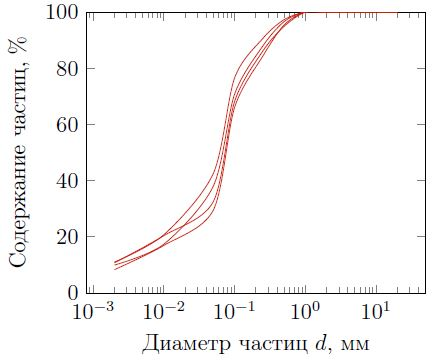
\includegraphics[width=0.25\linewidth]{6}}
%      \hfill
%      \subbottom[\label{fig:knuth_2-2}]{%
%          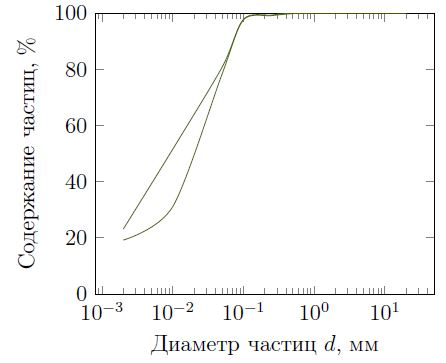
\includegraphics[width=0.25\linewidth]{7}}
%      \hfill
%      \subbottom[Третий подрисунок]{%
%          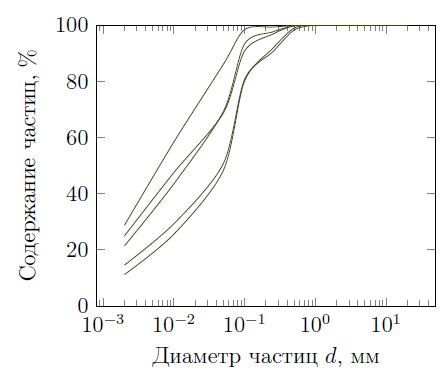
\includegraphics[width=0.3\linewidth]{8}}
%      \hfill
%  }
%  \legend{Подрисуночный текст, описывающий обозначения, например. Согласно
%  ГОСТ 2.105, пункт 4.3.1, располагается перед наименованием рисунка.}
%  \caption[Этот текст попадает в названия рисунков в списке рисунков]{Очень
%  длинная подпись к второму изображению, на~котором представлены две
%  фотографии Дональда Кнута}\label{fig:knuth_2}
%\end{figure}

Сопостовляя результаты рентгено-структурного анализа и гранулометрического, 
можно прийти к выводу, что содержание песка в образцах соотносится с 
содержанием кварца, пылеватых частиц --- плагиоклазов и калиевых
полевых шпатов, а содержание глинистых частиц примерно сопоставляется с 
содержанием иллита, смектита, каолинита, хлорита и других глинистых минералов.

\section{Физические свойства}

Результаты опытов по определению физических свойств представлены в 
Приложении \ref{app:phisics}. 

%\begin{sidewaystable}[p]
%  \centering
%   \begin{threeparttable}
%  \small
%  \caption{Физические свойства грунтов}
%   \label{tab:phis}
%  \begin{tabular}{|c|c|c|c|c|c|c|c|c|c|c|c|c|}
%    \toprule
%  Номер   образца & Глубина, \si{\meter} & Естественная   влажность, \% & Wl, \% & Wp, \% & Ip, \% & Il, д.е. & ρ, г/\si{\centi\meter^3} & ρs, г/\si{\centi\meter^3} & e, д.е. & Sr, д.е. & Наименование   грунта                        & ИГЭ \\ \hline
%  GJ6805          & 3,5        & 0,171                        & 0,238  & 0,134  & 0,105  & 0,36     & 2,17     & 2,72      & 0,471   & 0,987    & суглинок легкий   песчанистый тугопластичный & 6   \\ \hline
%  GJ6807          & 4,8        & 0,156                        & 0,228  & 0,129  & 0,099  & 0,27     & 2,17     & 2,69      & 0,449   & 0,945    & суглинок легкий   песчанистый тугопластичный & 6   \\ \hline
%  GJ6838          & 4,3        & 0,15                         & 0,20   & 0,11   & 0,09   & 0,41     & 2,18     & 2,68      & 0,415   & 0,96     & суглинок легкий   песчанистый тугопластичный & 6   \\ \hline
%  GJ6835          & 3,5        & 0,15                         & 0,20   & 0,11   & 0,09   & 0,36     & 2,17     & 2,72      & 0,433   & 0,91     & суглинок легкий   песчанистый тугопластичный & 6   \\ \hline
%  GJ6809          & 6          & 0,269                        & 0,322  & 0,21   & 0,112  & 0,53     & 1,97     & 2,72      & 0,752   & 0,973    & суглинок   мягкопластичный                   & 7   \\ \hline
%  GJ6810          & 6,4        & 0,251                        & 0,342  & 0,231  & 0,111  & 0,18     & 1,99     & 2,72      & 0,714   & 0,956    & суглинок полутвердый                         & 7   \\ \hline
%  GJ6821          & 6,7        & 0,233                        & 0,309  & 0,191  & 0,118  & 0,35     & 2,01     & 2,72      & 0,668   & 0,947    & суглинок   тугопластичный                    & 7   \\ \hline
%  GJ6898          & 12,1       & 0,24                         & 0,32   & 0,18   & 0,14   & 0,44     & 2,04     & 2,72      & 0,655   & 0,99     & суглинок тяжелый   пылеватый тугопластичный  & 7   \\ \hline
%  GJ6874          & 7,4        & 0,24                         & 0,34   & 0,18   & 0,16   & 0,34     & 2,01     & 2,72      & 0,675   & 0,96     & суглинок тяжелый   пылеватый тугопластичный  & 7   \\ \hline
%  GJ6888          & 10,2       & 0,23                         & 0,44   & 0,19   & 0,25   & 0,18     & 2,03     & 2,72      & 0,658   & 0,97     & глина легкая   пылеватая полутвердая         & 8   \\ \hline
%  GJ6890          & 10,6       & 0,22                         & 0,41   & 0,17   & 0,23   & 0,18     & 2,07     & 2,72      & 0,602   & 0,98     & глина легкая   песчанистая полутвердая       & 8   \\ \hline
%  GJ6852          & 10,3       & 0,21                         & 0,40   & 0,17   & 0,22   & 0,15     & 2,09     & 2,74      & 0,580   & 0,97     & глина полутвердая                            & 8   \\ \hline
%  GJ6889          & 10,4       & 0,22                         & 0,41   & 0,17   & 0,24   & 0,18     & 2,06     & 2,74      & 0,620   & 0,96     & глина полутвердая                            & 8   \\ \hline
%  GJ6822          & 8,3        & 0,244                        & 0,441  & 0,223  & 0,218  & 0,09     & 2,01     & 2,68      & 0,695   & 0,96     & глина полутвердая                            & 8   \\ \hline
%  GJ6884          & 9,2        & 0,22                         & 0,40   & 0,20   & 0,20   & 0,14     & 2,03     & 2,72      & 0,644   & 0,95     & глина легкая   пылеватая полутвердая         & 8   \\ \hline
%  GJ6846          & 8,3        & 0,21                         & 0,51   & 0,21   & 0,31   & 0,02     & 2,08     & 2,72      & 0,585   & 0,99     & глина тяжелая   полутвердая                  & 8   \\ \hline
%  GJ6855          & 11,7       & 0,192                        & 0,364  & 0,163  & 0,202  & 0,14     & 2,08     & 2,67      & 0,573   & 0,915    & глина легкая   песчанистая полутвердая       & 9   \\ \hline
%  GJ6859          & 12,5       & 0,187                        & 0,374  & 0,166  & 0,208  & 0,1      & 2,1      & 2,72      & 0,549   & 0,934    & глина полутвердая                            & 9   \\ \hline
%  GJ6865          & 14,7       & 0,156                        & 0,312  & 0,134  & 0,1788 & 0,12     & 2,18     & 2,72      & 0,442   & 0,944    & глина легкая   песчанистая полутвердая       & 9   \\ \hline
%  GJ68A3          & 13,5       & 0,18                         & 0,33   & 0,15   & 0,18   & 0,18     & 2,10     & 2,68      & 0,509   & 0,95     & глина легкая   песчанистая полутвердая       & 9   \\ \hline
%  GJ68B7          & 16,9       & 0,12                         & 0,30   & 0,13   & 0,17   & -0,06    & 2,26     & 2,72      & 0,354   & 0,94     & суглинок тяжелый   песчанистый твердый       & 9   \\ \hline
%  GJ68A7          & 14,6       & 0,13                         & 0,29   & 0,14   & 0,16   & 0,08     & 2,23     & 2,72      & 0,372   & 0,91     & суглинок твердый                             & 9   \\ \hline
%  GJ6856          & 11,9       & 0,21                         & 0,38   & 0,16   & 0,21   & 0,22     & 2,09     & 2,74      & 0,588   & 0,97     & глина полутвердая                            & 9   \\ \hline
%  GJ68A0          & 12,6       & 0,18                         & 0,32   & 0,14   &        &          & 2,13     & 2,71      & 0,499   &          & глина легкая   песчанистая полутвердая       & 9   \\ \hline
%  GJ6864          & 14,3       & 0,15                         & 0,31   & 0,14   & 0,17   & 0,06     & 2,19     & 2,72      & 0,433   & 0,97     & глина легкая   песчанистая полутвердая       & 9   \\ %\hline
%  \bottomrule 
%\end{tabular}
%   \end{threeparttable}
%  \end{sidewaystable}

В итоге по инженерно-геологическим элементам получились следующие 
средние значения плотности грунта: 6 ИГЭ --- 2,17 г/\si{\centi\meter^3}, 
7 ИГЭ --- 2,00 г/\si{\centi\meter^3}, 8 ИГЭ --- 2,05 г/\si{\centi\meter^3}, 
9 ИГЭ --- 2.15 г/\si{\centi\meter^3}; значения плотности твердых 
частиц: 6 ИГЭ --- 2,70 г/\si{\centi\meter^3}, 7 ИГЭ --- 2,72 
г/\si{\centi\meter^3}, 8 ИГЭ --- 2,72 г/\si{\centi\meter^3}, 
9 ИГЭ --- 2,71 г/\si{\centi\meter^3}. 
Средние значения верхнего и нижнего пределов пластичности 
получились такие: 6 ИГЭ --- 22 и 12 \% соответственно, 7 ИГЭ 
--- 33 и 20 \%, 8 ИГЭ --- 43 и 19 \%, 9 ИГЭ --- 33 и 15 \%.


\section{Параметры переуплотнения}

Проведя компрессионное сжатие для образцов грунтов, были построены 
графики в координатах $\sigma "--- e$ 
в полулогарифмическом масштабе и $\sigma "--- W$ для определения напряжения переуплотнения 
методами Казагранде и Беккера соответственно.

<<<<<<< HEAD
После построения графиков и их обработки, были определены 
напряжения предуплотнения $\sigma_c$, кПА,
они, в свою очередь, использовались для расчета 
других характеристик переуплотнения: напряжение 
переуплотнения $POP$ и коэффициент переуплотнения $OCR$.
Для расчетов также понадобился еще один показатель --- 
"бытовое" напряжение, получаемое по формуле \ref{eq:1}.
Результаты определений представлены в Таблице \ref{tab:komp}.
=======
Характеристики переуплотнения
представленны в таблице \ref{tab:komp}.
>>>>>>> b4dd3d04ae459e06fa2565cdcd3aae7f2e85c420

\begin{table}[]
  \centering
  \begin{threeparttable}
    \caption{Параметры переуплотнения}\label{tab:komp}
  \begin{tabular}{|c|c|c|c|c|}
  \hline
  Образец  & $\sigma_0$, \si{\kilo\Pa} & $\sigma_c$, \si{\kilo\Pa} & $POP$, \si{\kilo\Pa}   & $OCR$ \\ \hline
  GJ6809 & 118,2  & 300,0   & 181,8 & 2,5 \\ \hline
  GJ6822 & 166,8  & 475,0   & 308,2 & 2,8 \\ \hline
  GJ6810 & 127,4  & 480,0   & 352,6 & 3,8 \\ \hline
  GJ6821 & 134,7  & 455,0   & 320,3 & 3,4 \\ \hline
  GJ6805 &  76,0  & 225,0   & 149,1 & 3,0 \\ \hline
  GJ6807 & 104,2  & 390,0   & 285,8 & 3,7 \\ \hline
  GJ6855 & 243,4  & 455,0   & 211,6 & 1,9 \\ \hline
  GJ6859 & 262,5  & 510,0   & 247,5 & 1,9 \\ \hline
  GJ6865 & 320,5  & 600,0   & 279,5 & 1,9 \\ \hline
  GJ68A3 & 282,8  & 650,0   & 367,2 & 2,3 \\ \hline
  GJ6838 &  93,5  & 450,0   & 356,5 & 4,8 \\ \hline
  GJ6898 & 246,2  & 400,0   & 153,8 & 1,6 \\ \hline
  GJ6884 & 186,3  & 780,0   & 593,7 & 4,2 \\ \hline
  GJ6846 & 172,6  & 290,0   & 117,4 & 1,7 \\ \hline
  \end{tabular}
\end{threeparttable}
  \end{table}

